%======================================================================
% GMI-05 Tenzory.pdf
%======================================================================
% grafické značení tenzorů: krabička s nožičkami
%   \gmIpetT{T}{posun/typ,...}{posun/typ,...}  nahoře / dole, typ s = rovná, w = vlnitá
% (babel czech dělá z "-" aktivní znak -> definice maker s TikZ souřadnicemi musí být s \shorthandoff{-})
\shorthandoff{-}%
\tikzset{gmIpets/.style={},gmIpetw/.style={decorate,decoration={snake,amplitude=0.8pt,segment length=2.5pt}}}
\providecommand{\gmIpetT}[3]{\tikz[baseline=(gmb.base),line width=0.5pt]{%
  \node[draw,inner sep=1.2pt,minimum width=1.2em,minimum height=1.1em] (gmb) {$\scriptstyle #1$};%
  \foreach \o/\t in {#2}{\draw[gmIpet\t] ($(gmb.north)+(\o em,0)$) -- ++(0,0.7em);}%
  \foreach \o/\t in {#3}{\draw[gmIpet\t] ($(gmb.south)+(\o em,0)$) -- ++(0,-0.7em);}}}
\shorthandon{-}%

\section{Tenzory a tenzorová pole}
\strana{GMI-05-1}

\begin{itemize}[nosep]
  \item Tenzorový součin
  \item Značení tenzorů
  \item Operace na tenzorových prostorech
  \item Souřadnice tenzorů
  \item Tenzory -- univerzální lineární zobrazení
  \item Tenzorová pole
  \item Tenzorové derivace
\end{itemize}

%----------------------------------------------------------------------
\strana{GMI-05-2}
\subsection{Tenzorový součin}

\begin{definice}[Tenzorový součin]
mějme vekt.\ pr.\ $V_1,\dots,V_k$ nad $\mathbb{K}$ \\
\kw{tenzorový součin} $V_1\otimes\dots\otimes V_k$ je prostor lin.\ kombinací formálních součinů prvků z $V_i$ s uvážením linearity v každém z arg.\ (distrib.\ a asoc.\ náš.\ skal.)

konkrétně
\[
  V_1\otimes\dots\otimes V_k = \mathrm{Free}[V_1\times\dots\times V_k]\,/\,U_0
\]
\begin{itemize}[nosep]
  \item[] $\mathrm{Free}[V_1\times\dots\times V_k]$ \quad volný vekt.\ pr.\ generovaný formálními lin.\ kombinacemi prvků z $V_1\times\dots\times V_k$
  \item[] $U_0$ \quad vekt.\ pr.\ generovaný form.\ lin.\ kombinacemi prvků z $\mathrm{Free}[V_1\times\dots\times V_k]$ typu
  \begin{align*}
    &[a_1,\dots,\alpha a_j,\dots,a_k] - \alpha[a_1,\dots,a_j,\dots,a_k] \\
    &[a_1,\dots,u+v,\dots,a_k] - [a_1,\dots,u,\dots,a_k] - [a_1,\dots,v,\dots,a_k]
  \end{align*}
\end{itemize}
píšeme
\[
  \vzorec{a_1\otimes\dots\otimes a_k = [a_1,\dots,a_k]_{U_0}}
\]
\end{definice}

\begin{vysvetleni}[Co dělá faktorizace podle $U_0$]
Ve volném prostoru $\mathrm{Free}[V_1\times\dots\times V_k]$ jsou všechny $k$-tice $[a_1,\dots,a_k]$ lineárně nezávislé (i $[2a_1,a_2]$ a $2[a_1,a_2]$ jsou různé prvky) -- prostor je obrovský. Faktorizací podle $U_0$ prohlásíme za nulové přesně ty kombinace, které by porušily linearitu v jednotlivých argumentech; třída $a_1\otimes\dots\otimes a_k$ je pak multilineární v každém $a_j$ (např.\ $(\alpha a)\otimes b=\alpha(a\otimes b)=a\otimes(\alpha b)$). Důsledek (\uv{univerzální vlastnost}): multilineární zobrazení z $V_1\times\dots\times V_k$ odpovídají lineárním zobrazením z $V_1\otimes\dots\otimes V_k$. Pro konečnou dimenzi tvoří báze $e^{(1)}_{i_1}\otimes\dots\otimes e^{(k)}_{i_k}$, tj.\ $\dim = \prod_j\dim V_j$. Obecný tenzor \emph{není} součinový, je jen součtem součinových (např.\ $e_1\otimes e_1+e_2\otimes e_2$).
\end{vysvetleni}

\underline{Pozn:} stejné def.\ lze dát i pro součin $R$-modulů \\
\quad píšeme $V_1\otimes_R V_2\otimes_R\dots$ \quad pokud je potřeba zdůraznit $R$

\underline{Pozn:} často budeme uvažovat vekt.\ pr.\ (modul) $V$ a jeho duál $V^*$ \\
\quad vždy budeme předpokládat \kw{reflexivitu}, tj.\ $V = V^{**}$ \\
\quad splněno pro kon.\ dim.\ vekt.\ pr.\ či lokálně kon.\ gener.\ moduly

existují přirozené isomorfismy typu
\[
  \begin{aligned}
    (U\otimes V)\otimes W &\leftrightarrow U\otimes V\otimes W \\
    U\otimes V &\leftrightarrow V\otimes U
  \end{aligned}
  \qquad\qquad
  \begin{aligned}
    (u\otimes v)\otimes w &\leftrightarrow u\otimes v\otimes w \\
    u\otimes v &\leftrightarrow v\otimes u
  \end{aligned}
\]
budeme nazývat stejného typu a ztotožňovat \\
pro $U, V, W$ různé nemůže vést k nedorozumění a můžeme psát \\
\quad $(u\otimes v)\otimes w = u\otimes v\otimes w$ \qquad $u\otimes v = v\otimes u$ \\
\pozor{pro $U = V$ může v $V\otimes V$ dojít k nedorozumění} \\
\quad $u\otimes v$ a $v\otimes u$ reprez.\ dva různé tenzory \\
\quad isomorf.\ $U\otimes V$ s $V\otimes U$, \ $u\otimes v\leftrightarrow v\otimes u$ \ pouze říká, že záměnou dostaneme isomorf.\ pr., ne že $u\otimes v = v\otimes u$ \\
\quad musíme umět rozlišit, do kt.\ činitele součinu $V\otimes V$ patří jednotlivé vektory v $u\otimes v$

%----------------------------------------------------------------------
\strana{GMI-05-3}
\subsection{Značení tenzorů}
\providecommand{\gmIpa}{\underline{a}}
\providecommand{\gmIpb}{\underline{b}}
\providecommand{\gmIpc}{\underline{c}}
\providecommand{\gmIpA}{\underline{\mathsf{A}}}
\providecommand{\gmIpB}{\underline{\mathsf{B}}}

\textbf{abstraktní značení} \\
\quad příslušnost vektorů v součinu do jedn.\ činitelů tenz.\ součinu určujeme důsledně pořadím
\[
  u\otimes v\otimes\phi \;\in\; \underset{\textstyle\overset{\uparrow}{u}}{V}\otimes\underset{\textstyle\overset{\uparrow}{v}}{V}\otimes\underset{\textstyle\overset{\uparrow}{\phi}}{U}
\]
\quad v tomto pojetí je násobení v $V\otimes V$ nekomutativní \quad $u\otimes v\neq v\otimes u$

\textbf{značení pomocí abstraktních indexů}
\begin{itemize}[nosep]
  \item[] každý prostor v tenz.\ součinu pojmenujeme abstr.\ indexem \\
          stejné prostory indexem stejného typu
  \[
    \underset{\gmIpa}{V}\otimes\underset{\gmIpb}{V}\otimes\underset{\gmIpA}{U}
    \qquad\text{používáme podtržená písmenka různých typů (font, abeceda, velikost)}
  \]
  \item[] vekt.\ z $U, V$ mají 1 index, např.\ $u^{\gmIpa}$, $\phi^{\gmIpA}$ \\
          tenzory z tenz.\ souč.\ mají příslušný počet indexů, \ např.\ $T^{\gmIpa\gmIpb\gmIpA}\in V\otimes V\otimes U$
  \item[] pro součinové tenz.\ defaultně rozumíme
          \[ (u\otimes v\otimes\phi)^{\gmIpa\gmIpb\gmIpA} = u^{\gmIpa}\otimes v^{\gmIpb}\otimes\phi^{\gmIpA} \]
  \item[] duální prostory označujeme indexy stejného typu umístěnými dole \quad
          $\phi^{\gmIpA}\in U$, \ $\psi_{\gmIpA}\in U^*$
  \item[] pojmenování činitelů umožňuje uvolnit pořadí v tenz.\ násobení -- formální komutativita
  \[
    u^{\gmIpa}\otimes v^{\gmIpb} = v^{\gmIpb}\otimes u^{\gmIpa}
    \ \underset{\text{\scriptsize$\uparrow$ obecně}}{\neq}\
    v^{\gmIpa}\otimes u^{\gmIpb} = u^{\gmIpb}\otimes v^{\gmIpa}
  \]
\end{itemize}

\begin{vysvetleni}[Abstraktní indexy]
Podtržený index ($\underline a,\underline b,\underline{\mathsf A},\dots$) \emph{není} číslo složky a neprobíhá hodnoty $1,\dots,d$ -- je to jen jmenovka \uv{slotu} (činitele tenzorového součinu), do kterého daný vektor patří. $T^{\underline a\underline b\underline{\mathsf A}}$ je tedy stále celý tenzor, nezávislý na bázi. Horní index = slot z $V$ (vektor), dolní = slot z $V^*$ (forma); typ písmene (latinka, bezpatkové velké, \dots) rozlišuje různé prostory $V$, $U$. Protože sloty jsou pojmenované, nezáleží na pořadí zápisu činitelů ($u^{\underline a}v^{\underline b}=v^{\underline b}u^{\underline a}$), ale záleží na tom, \emph{který} vektor nese který index ($u^{\underline a}v^{\underline b}\neq v^{\underline a}u^{\underline b}$). Stejný horní a dolní index znamená kontrakci (viz níže). Krtouš (odd.\ 1.2) píše abstraktní indexy tučně místo podtržení; souřadnicové indexy jsou obyčejné (nepodtržené).
\end{vysvetleni}

\textbf{grafické značení}
\begin{itemize}[nosep]
  \item[] každý prostor v tenz.\ součinu má svou vlastní nožičku \\
          stejné prostory mají stejné nožičky, duál orient.\ dolů
\end{itemize}
\[
  \begin{array}{lll@{\qquad}ll}
    V & \text{vektory} & \gmIpetT{u}{0/s}{},\ \gmIpetT{v}{0/s}{} & V^*\ \text{1-formy} & \gmIpetT{\alpha}{}{0/s}\ \ \gmIpetT{\beta}{}{0/s} \\[10pt]
    U & \text{vektory} & \gmIpetT{\phi}{0/w}{},\ \gmIpetT{\psi}{0/w}{} & U^*\ \text{1-formy} & \gmIpetT{\sigma}{}{0/w}\ \ \gmIpetT{\omega}{}{0/w}
  \end{array}
\]
tenzory z tenz.\ součinů \qquad $\gmIpetT{T}{-0.3/s,0/s,0.3/w}{} \;\in\; V\otimes V\otimes U$

identifikace tenz.\ činitelů se dělá pořadím nožiček
\[
  \gmIpetT{T}{-0.3/s,0/s,0.3/w}{} \;=\; \gmIpetT{u}{0/s}{}\ \gmIpetT{v}{0/s}{}\ \gmIpetT{\phi}{0/w}{}
\]
lze měnit pořadí symbolů při zachování pořadí nožiček
\[
  \gmIpetT{u}{0/s}{}\ \gmIpetT{v}{0/s}{}
  \;=\;
  \tikz[baseline=(gx.base),line width=0.5pt]{%
    \node[draw,inner sep=1.2pt,minimum width=1.2em,minimum height=1.1em] (gx) at (0,0) {$\scriptstyle v$};
    \node[draw,inner sep=1.2pt,minimum width=1.2em,minimum height=1.1em] (gy) at (1.8em,0) {$\scriptstyle u$};
    \draw (gx.north) -- ++(0.9em,0.7em) -- ++(0.9em,0.25em);
    \draw (gy.north) -- ++(-0.9em,0.7em) -- ++(-0.9em,0.25em);}
  \ \underset{\text{\scriptsize$\uparrow$ obecně}}{\neq}\
  \gmIpetT{v}{0/s}{}\ \gmIpetT{u}{0/s}{}
  \;=\;
  \tikz[baseline=(gx.base),line width=0.5pt]{%
    \node[draw,inner sep=1.2pt,minimum width=1.2em,minimum height=1.1em] (gx) at (0,0) {$\scriptstyle u$};
    \node[draw,inner sep=1.2pt,minimum width=1.2em,minimum height=1.1em] (gy) at (1.8em,0) {$\scriptstyle v$};
    \draw (gx.north) -- ++(0.9em,0.7em) -- ++(0.9em,0.25em);
    \draw (gy.north) -- ++(-0.9em,0.7em) -- ++(-0.9em,0.25em);}
\]

\begin{vysvetleni}[Jak číst diagramy \uv{krabička s nožičkami}]
Jde o grafickou obdobu abstraktních indexů (tzv.\ Penroseova grafická notace):
\begin{itemize}[nosep,leftmargin=1.2em]
  \item \textbf{krabička} = tenzor, \textbf{nožička} = jeden slot (jeden abstraktní index);
  \item nožička \textbf{nahoru} = horní index (slot z $V$, vektorový), nožička \textbf{dolů} = dolní index (slot z $V^*$, formový);
  \item \textbf{druh čáry} rozlišuje prostory: rovná = $V$, vlnitá = $U$ (odpovídá různým typům písmen u indexů);
  \item \textbf{pořadí volných konců zleva doprava} (nahoře) určuje, do kterého činitele součinu slot patří -- hraje roli jména indexu; krabičky samotné lze libovolně přeskládat, pokud konce nožiček zůstanou na svých místech (proto se nožičky překříží);
  \item krabičky vedle sebe = tenzorový součin, \textbf{spojená} horní a dolní nožička = kontrakce (sčítací index), samotná čára bez krabičky = jednotkový tenzor $\delta$ (viz dále).
\end{itemize}
Tedy např.\ dvě krabičky $u$, $v$ se zkříženými nožičkami jsou $v\otimes u$ zapsané \uv{pozpátku}: levý slot nese $v$, pravý $u$.
\end{vysvetleni}

%----------------------------------------------------------------------
\strana{GMI-05-4}
% dvě krabičky se zkříženými nožičkami
\shorthandoff{-}%
\providecommand{\gmIpetX}[2]{\tikz[baseline=(gx.base),line width=0.5pt]{%
    \node[draw,inner sep=1.2pt,minimum width=1.2em,minimum height=1.1em] (gx) at (0,0) {$\scriptstyle #1$};
    \node[draw,inner sep=1.2pt,minimum width=1.2em,minimum height=1.1em] (gy) at (1.8em,0) {$\scriptstyle #2$};
    \draw (gx.north) -- ++(0.9em,0.7em) -- ++(0.9em,0.25em);
    \draw (gy.north) -- ++(-0.9em,0.7em) -- ++(-0.9em,0.25em);}}
\shorthandon{-}%

\textbf{porovnání značení} \qquad $u, v\in V$, \quad $\phi\in U$, \qquad $X, Y\in V\otimes V\otimes U$

abstraktní znač.
\begin{align*}
  X &= u\otimes v\otimes\phi && = \phi\otimes u\otimes v \\
  Y &= v\otimes u\otimes\phi && = \phi\otimes v\otimes u
\end{align*}
značení pomocí abstr.\ indexů
\begin{align*}
  X^{\gmIpa\gmIpb\gmIpA} &= u^{\gmIpa}v^{\gmIpb}\phi^{\gmIpA} = v^{\gmIpb}u^{\gmIpa}\phi^{\gmIpA} = \phi^{\gmIpA}u^{\gmIpa}v^{\gmIpb} \\
  Y^{\gmIpa\gmIpb\gmIpA} &= v^{\gmIpa}u^{\gmIpb}\phi^{\gmIpA} = u^{\gmIpb}v^{\gmIpa}\phi^{\gmIpA} = \phi^{\gmIpA}v^{\gmIpa}u^{\gmIpb}
\end{align*}
grafické značení
\begin{align*}
  \gmIpetT{X}{-0.3/s,0/s,0.3/w}{} &= \gmIpetT{u}{0/s}{}\ \gmIpetT{v}{0/s}{}\ \gmIpetT{\phi}{0/w}{}
   = \gmIpetX{v}{u}\ \gmIpetT{\phi}{0/w}{}
   = \gmIpetT{\phi}{0/w}{}\ \gmIpetT{u}{0/s}{}\ \gmIpetT{v}{0/s}{} \\[4pt]
  \gmIpetT{Y}{-0.3/s,0/s,0.3/w}{} &= \gmIpetT{v}{0/s}{}\ \gmIpetT{u}{0/s}{}\ \gmIpetT{\phi}{0/w}{}
   = \gmIpetX{u}{v}\ \gmIpetT{\phi}{0/w}{}
   = \gmIpetT{\phi}{0/w}{}\ \gmIpetT{v}{0/s}{}\ \gmIpetT{u}{0/s}{}
\end{align*}

obvykle vynecháváme znaménko $\otimes$ \qquad $u\otimes v = uv$ \qquad $u\otimes v\otimes\phi = uv\phi$

\begin{definice}[tenzory nad $V$]
\[
  V^k_l = \underbrace{V\otimes\dots\otimes V}_{k}\otimes\underbrace{V^*\otimes\dots\otimes V^*}_{l}
  \quad\text{je \kw{tenz.\ mocnina} $V$ typu $(k,l)$}
\]
\quad $k$-krát kontravariantní, \ $l$-krát kovariantní \\
\quad $A\in V^k_l$ \ \kw{tenzor typu $(k,l)$}
\end{definice}

\begin{vysvetleni}[Porovnání tří značení; typ $(k,l)$]
$X$ a $Y$ se liší jen tím, který z vektorů $u,v$ sedí v prvním a který ve druhém slotu $V$; ve všech třech zápisech je proto $X\neq Y$ (obecně), ale přeskládání zápisu při zachování přiřazení slotů nic nemění. Abstraktní značení drží přiřazení pořadím, indexové jménem indexu, grafické polohou konce nožičky. Tenzor typu $(k,l)$ má $k$ horních (kontravariantních) a $l$ dolních (kovariantních) indexů, tj.\ $k$ nožiček nahoru a $l$ dolů; Krtouš značí $V^p_q$ stejně (rov.\ (1.1)).
\end{vysvetleni}

%----------------------------------------------------------------------
\strana{GMI-05-5}
\tikzset{gmIpetbox/.style={draw,inner sep=1.2pt,minimum width=1.2em,minimum height=1.1em}}
\subsection{Operace na tenzorových prostorech}

Lineární operace lze rozšířit z jejich znalosti na součinových tenzorech \\
\quad $\Leftarrow$ obecný tenzor je lin.\ kombinace součinových tenz.

\subsubsection*{Zúžení, kontrakce}
zúžení mezi $V^*$ a $V$ lze rozšířit na lib.\ tenz.\ součin obsahující $V^*\otimes V$

\begin{definice}[Kontrakce]
mějme $V^k_l$, \ pro součinové tenz.\ def.
\[
  \mathsf{C}^p_q: V^k_l\to V^{k-1}_{l-1}
\]
\[
  u_1\otimes\dots\otimes u_k\otimes\alpha^1\otimes\dots\otimes\alpha^l
  \;\to\; (\alpha^q\cdot u_p)\,
  \underbrace{u_1\otimes\dots\otimes u_k}_{\text{mimo } u_p}\otimes
  \underbrace{\alpha^1\otimes\dots\otimes\alpha^l}_{\text{mimo } \alpha^q}
\]
rozšíříme na celé $V^k_l$ linearitou
\end{definice}

\begin{minipage}{0.62\textwidth}
značení
\[
  \mathsf{C}^p_q\,T \qquad\qquad
  T^{\overset{\scriptstyle\text{\scriptsize$p$-tá pozice}}{\overset{\downarrow}{\phantom{m}}}}{}
  \;\equiv\;
  T^{\underline{a}_1\dots\underline{m}\dots\underline{a}_k}{}_{\underline{b}_1\dots\underline{m}\dots\underline{b}_l}
\]
\hspace*{4.6cm}{\small $\uparrow$ $q$-tá pozice (dolní $\underline{m}$)}
\end{minipage}
\begin{minipage}{0.36\textwidth}
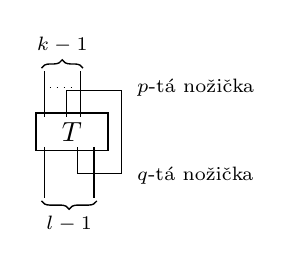
\begin{tikzpicture}[line width=0.5pt,x=1em,y=1em]
  \node[draw,minimum width=2.6em,minimum height=1.1em] (T) at (0,0) {$T$};
  % horní nožičky (k-1)
  \draw (-1,0.55) -- (-1,2.2);
  \draw (0.3,0.55) -- (0.3,2.2);
  \draw[dotted] (-0.8,1.6) -- (0.1,1.6);
  % p-tá nožička se smyčkou
  \draw (-0.2,0.55) -- (-0.2,1.5) -- (1.8,1.5) -- (1.8,-1.5) -- (0.2,-1.5) -- (0.2,-0.55);
  % dolní nožičky (l-1)
  \draw (-1,-0.55) -- (-1,-2.4);
  \draw (0.8,-0.55) -- (0.8,-2.4);
  \draw[decorate,decoration={brace,amplitude=3pt}] (-1.1,2.3) -- (0.4,2.3) node[midway,above=2pt] {\scriptsize $k-1$};
  \draw[decorate,decoration={brace,amplitude=3pt,mirror}] (-1.1,-2.5) -- (0.9,-2.5) node[midway,below=2pt] {\scriptsize $l-1$};
  \node[right,font=\scriptsize] at (2,1.6) {$p$-tá nožička};
  \node[right,font=\scriptsize] at (2,-1.6) {$q$-tá nožička};
\end{tikzpicture}
\end{minipage}

tj.
\[
  \begin{array}{l@{\qquad}l@{\qquad}c}
    \alpha\cdot a & \alpha_{\underline{m}}a^{\underline{m}} &
      \tikz[baseline=-0.6ex,line width=0.5pt]{\node[gmIpetbox] (x) at (0,0.45) {$\scriptstyle\alpha$}; \node[gmIpetbox] (y) at (0,-0.45) {$\scriptstyle a$}; \draw (x.south) -- (y.north);} \\[18pt]
    \mathsf{C}A = \operatorname{tr}A & A^{\underline{m}}{}_{\underline{m}} &
      \tikz[baseline=-0.6ex,line width=0.5pt]{\node[gmIpetbox] (x) at (0,0) {$\scriptstyle A$}; \draw (x.north) -- ++(0,0.25) -- ++(0.45,0) -- ++(0,-0.95) -- ++(-0.45,0) -- (x.south);} \\[18pt]
    A\cdot a & A^{\underline{a}}{}_{\underline{m}}a^{\underline{m}} &
      \tikz[baseline=-0.6ex,line width=0.5pt]{\node[gmIpetbox] (x) at (0,0.45) {$\scriptstyle A$}; \node[gmIpetbox] (y) at (0,-0.45) {$\scriptstyle a$}; \draw (x.south) -- (y.north); \draw (x.north) -- ++(0,0.3);} \\[22pt]
    A\cdot B = C & C^{\underline{a}}{}_{\underline{b}} = A^{\underline{a}}{}_{\underline{m}}B^{\underline{m}}{}_{\underline{b}} &
      \tikz[baseline=-0.6ex,line width=0.5pt]{\node[gmIpetbox] (c) at (0,0) {$\scriptstyle C$}; \draw (c.north) -- ++(0,0.3); \draw (c.south) -- ++(0,-0.3);}
      \ = \
      \tikz[baseline=-0.6ex,line width=0.5pt]{\node[gmIpetbox] (x) at (0,0.45) {$\scriptstyle A$}; \node[gmIpetbox] (y) at (0,-0.45) {$\scriptstyle B$}; \draw (x.south) -- (y.north); \draw (x.north) -- ++(0,0.3); \draw (y.south) -- ++(0,-0.3);}
  \end{array}
\]

\begin{vysvetleni}[Kontrakce]
Kontrakce $\mathsf C^p_q$ \uv{spáruje} $p$-tý vektorový slot s $q$-tým formovým slotem pomocí přirozeného zúžení $\alpha\cdot u$; typ klesne z $(k,l)$ na $(k-1,l-1)$. Definice na součinových tenzorech stačí, protože každý tenzor je jejich lineární kombinací a výsledek je lineární. V indexech: stejné jméno nahoře a dole ($\underline m$), v grafice: $p$-tá horní nožička se ohne a napojí na $q$-tou dolní. Tabulka ukazuje známé případy: zúžení formy s vektorem (krabička $\alpha$ \uv{sedí} na nožičce $a$), stopa matice ($A$ s nožičkou spojenou sama se sebou), působení matice na vektor a maticové násobení (svislé řetězení krabiček). V bázi to jsou přesně $\alpha_ja^j$, $A^j{}_j$, $A^i{}_ja^j$, $A^i{}_jB^j{}_k$.
\end{vysvetleni}

\textbf{jednotkový tenzor}
\[
  \delta\in V^1_1 \qquad \delta^{\underline{a}}{}_{\underline{b}} \qquad
  \tikz[baseline=-0.6ex,line width=0.5pt]{\draw (0,-0.4) -- (0,0.4);}
\]
reprezentuje identickou transf.
\[
  \begin{array}{l@{\qquad}l@{\qquad}c}
    \delta\cdot a = a & \delta^{\underline{a}}{}_{\underline{m}}a^{\underline{m}} = a^{\underline{a}} &
      \tikz[baseline=-0.6ex,line width=0.5pt]{\node[gmIpetbox] (y) at (0,-0.2) {$\scriptstyle a$}; \draw (y.north) -- ++(0,0.6);}
      \ = \ \gmIpetT{a}{0/s}{} \\[14pt]
    \mathsf{C}\delta = d & \delta^{\underline{m}}{}_{\underline{m}} = d &
      \tikz[baseline=-0.6ex,line width=0.5pt]{\draw (0,0) ellipse (0.12 and 0.4);} \ = d
  \end{array}
\]

\begin{vysvetleni}[Jednotkový tenzor]
$\delta\in V\otimes V^*$ je tenzor odpovídající identitě $V\to V$ (v bázi $\delta^i{}_j$ = Kroneckerovo delta, $\delta=e_i\otimes e^i$). Graficky je to holá čára: připojit ji k nožičce nic nezmění (\uv{čáru lze prodloužit}). Uzavřená smyčka je stopa identity, tj.\ $\delta^{\underline m}{}_{\underline m}=d=\dim V$.
\end{vysvetleni}

%----------------------------------------------------------------------
\strana{GMI-05-6}
\shorthandoff{-}%
% krabička se 3 nožičkami permutovanými: \gmIpetPerm{i,j,k} -- nožička z pozice 1,2,3 jde na pozici i,j,k
\providecommand{\gmIpetPerm}[1]{\tikz[baseline=-0.6ex,line width=0.5pt,x=1em,y=1em]{%
  \draw (-0.9,-0.5) rectangle (0.9,0.5);
  \foreach \t [count=\s] in {#1}{\draw (-1.2+0.6*\s,0.5) -- (-1.2+0.6*\t,1.4);}}}
% krabička T se 3 nožičkami a pruhem (sym. = vlnitý, antisym. = rovný)
\providecommand{\gmIpetSym}[2]{\tikz[baseline=-0.6ex,line width=0.5pt,x=1em,y=1em]{%
  \draw (-0.9,-0.5) rectangle (0.9,0.5); \node at (0,0) {$\scriptstyle #1$};
  \foreach \s in {1,2,3}{\draw (-1.2+0.6*\s,0.5) -- (-1.2+0.6*\s,1.5);}
  \draw[#2] (-1.05,1.0) -- (1.05,1.0);}}
\tikzset{gmIpetsymbar/.style={decorate,decoration={snake,amplitude=1pt,segment length=3pt}},gmIpetasymbar/.style={line width=1pt}}
\shorthandon{-}%

\textbf{permutace na $V^k$} \\
\quad $\sigma$ permutace čísel $1\dots k$, \quad $\bar\sigma$ inverzní perm.
\[
  P_\sigma\,u_1\otimes\dots\otimes u_k = u_{\bar\sigma_1}\otimes\dots\otimes u_{\bar\sigma_k}
\]
pomocí abstr.\ indexů
\[
  \vzorec{(P_\sigma T)^{\underline{a}_1\dots\underline{a}_k} = T^{\underline{a}_{\sigma_1}\dots\underline{a}_{\sigma_k}}}
\]
\quad ověření: \quad
$(P_\sigma\,u_1\otimes\dots\otimes u_k)^{\underline{a}_1\dots\underline{a}_k}
 = u_{\bar\sigma_1}^{\underline{a}_1}\otimes\dots\otimes u_{\bar\sigma_k}^{\underline{a}_k}
 = u_1^{\underline{a}_{\sigma_1}}\otimes\dots\otimes u_k^{\underline{a}_{\sigma_k}}$

grafické zn.
\begin{center}
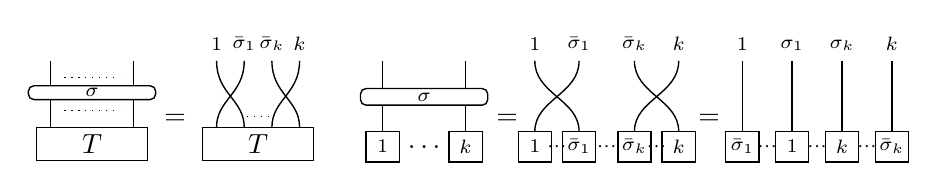
\begin{tikzpicture}[line width=0.5pt,x=1em,y=1em]
  % P_sigma T
  \draw (0,0) rectangle (4,1.2); \node at (2,0.6) {$T$};
  \draw (0.5,1.2) -- (0.5,3.6); \draw (3.5,1.2) -- (3.5,3.6);
  \draw[dotted] (1,1.8) -- (3,1.8); \draw[dotted] (1,3.0) -- (3,3.0);
  \draw[fill=white,rounded corners=2pt] (-0.3,2.2) rectangle (4.3,2.7); \node at (2,2.45) {$\scriptstyle\sigma$};
  \node at (5,1.5) {$=$};
  \begin{scope}[xshift=6em]
    \draw (0,0) rectangle (4,1.2); \node at (2,0.6) {$T$};
    \draw (0.5,1.2) .. controls (0.5,2.2) and (1.5,2.4) .. (1.5,3.6);
    \draw (1.5,1.2) .. controls (1.5,2.2) and (0.5,2.4) .. (0.5,3.6);
    \draw (2.5,1.2) .. controls (2.5,2.2) and (3.5,2.4) .. (3.5,3.6);
    \draw (3.5,1.2) .. controls (3.5,2.2) and (2.5,2.4) .. (2.5,3.6);
    \draw[dotted] (1.6,1.6) -- (2.4,1.6);
    \node[above,font=\scriptsize] at (0.5,3.6) {$1$}; \node[above,font=\scriptsize] at (1.5,3.6) {$\bar\sigma_1$};
    \node[above,font=\scriptsize] at (2.5,3.6) {$\bar\sigma_k$}; \node[above,font=\scriptsize] at (3.5,3.6) {$k$};
  \end{scope}
  % P_sigma u_1 ... u_k
  \begin{scope}[xshift=12em]
    \node[gmIpetbox] (a) at (0.5,0.5) {$\scriptstyle 1$}; \node[gmIpetbox] (b) at (3.5,0.5) {$\scriptstyle k$};
    \node at (2,0.5) {$\dots$};
    \draw (a.north) -- (0.5,3.6); \draw (b.north) -- (3.5,3.6);
    \draw[fill=white,rounded corners=2pt] (-0.3,2.0) rectangle (4.3,2.6); \node at (2,2.3) {$\scriptstyle\sigma$};
    \node at (5,1.5) {$=$};
  \end{scope}
  \begin{scope}[xshift=18em]
    \foreach \x/\l in {0/1,1.6/\bar\sigma_1,3.6/\bar\sigma_k,5.2/k}{\node[gmIpetbox] at (\x,0.5) {$\scriptstyle\l$};}
    \node at (0.8,0.5) {$\scriptstyle\cdots$}; \node at (2.6,0.5) {$\scriptstyle\cdots$}; \node at (4.4,0.5) {$\scriptstyle\cdots$};
    \draw (0,1.05) .. controls (0,2.2) and (1.6,2.4) .. (1.6,3.6);
    \draw (1.6,1.05) .. controls (1.6,2.2) and (0,2.4) .. (0,3.6);
    \draw (3.6,1.05) .. controls (3.6,2.2) and (5.2,2.4) .. (5.2,3.6);
    \draw (5.2,1.05) .. controls (5.2,2.2) and (3.6,2.4) .. (3.6,3.6);
    \node[above,font=\scriptsize] at (0,3.6) {$1$}; \node[above,font=\scriptsize] at (1.6,3.6) {$\bar\sigma_1$};
    \node[above,font=\scriptsize] at (3.6,3.6) {$\bar\sigma_k$}; \node[above,font=\scriptsize] at (5.2,3.6) {$k$};
    \node at (6.3,1.5) {$=$};
  \end{scope}
  \begin{scope}[xshift=25.5em]
    \foreach \x/\l/\u in {0/\bar\sigma_1/1,1.8/1/\sigma_1,3.6/k/\sigma_k,5.4/\bar\sigma_k/k}{\node[gmIpetbox] at (\x,0.5) {$\scriptstyle\l$}; \draw (\x,1.05) -- (\x,3.6); \node[above,font=\scriptsize] at (\x,3.6) {$\u$};}
    \node at (0.9,0.5) {$\scriptstyle\cdots$}; \node at (2.7,0.5) {$\scriptstyle\cdots$}; \node at (4.5,0.5) {$\scriptstyle\cdots$};
  \end{scope}
\end{tikzpicture}
\end{center}

\begin{definice}[Symetrizace na $V^k$]
\[
  \mathcal{S}\,T = \frac{1}{k!}\sum_{\substack{\sigma\\ \text{perm.\,}1\dots k}} P_\sigma T
  \qquad\qquad
  (\mathcal{S}T)^{\underline{a}_1\dots\underline{a}_k} = \vzorec{T^{(\underline{a}_1\dots\underline{a}_k)}} = \frac{1}{k!}\sum_\sigma T^{\underline{a}_{\sigma_1}\dots\underline{a}_{\sigma_k}}
\]
\end{definice}
\[
  \gmIpetSym{T}{gmIpetsymbar}
  \qquad\text{např.}\qquad
  \gmIpetSym{}{gmIpetsymbar} = \frac16\Big(\gmIpetPerm{1,2,3} + \gmIpetPerm{2,3,1} + \gmIpetPerm{3,1,2} + \gmIpetPerm{2,1,3} \oprava{+}{-} \gmIpetPerm{3,2,1} + \gmIpetPerm{1,3,2}\Big)
\]

\begin{definice}[Antisymetrizace na $V^k$]
\[
  \mathcal{A}\,T = \frac{1}{k!}\sum_\sigma \operatorname{sign}\sigma\; P_\sigma T
  \qquad\qquad
  (\mathcal{A}T)^{\underline{a}_1\dots\underline{a}_k} = \vzorec{T^{[\underline{a}_1\dots\underline{a}_k]}} = \frac{1}{k!}\sum_\sigma \operatorname{sign}\sigma\; T^{\underline{a}_{\sigma_1}\dots\underline{a}_{\sigma_k}}
\]
\end{definice}
\[
  \gmIpetSym{T}{gmIpetasymbar}
  \qquad\text{např.}\qquad
  \gmIpetSym{}{gmIpetasymbar} = \frac16\Big(\gmIpetPerm{1,2,3} + \gmIpetPerm{2,3,1} + \gmIpetPerm{3,1,2} - \gmIpetPerm{1,3,2} - \gmIpetPerm{3,2,1} - \gmIpetPerm{2,1,3}\Big)
\]

\begin{vysvetleni}[Permutace, (anti)symetrizace a jejich diagramy]
$P_\sigma$ přehazuje pořadí \uv{slotů} (nožiček) tenzoru; v abstraktních indexech prostě přejmenuje indexy, $(P_\sigma T)^{\underline a_1\dots\underline a_k}=T^{\underline a_{\sigma_1}\dots\underline a_{\sigma_k}}$. Na součinovém tenzoru je proto na pozici $i$ vektor $u_{\bar\sigma_i}$ (inverzní permutace) -- odtud řádek \uv{ověření}. V diagramech je permutace jen překřížení nožiček (obdélník $\sigma$ = \uv{přepojovací box}).

Symetrizace $\mathcal S$ a antisymetrizace $\mathcal A$ jsou projektory ($\mathcal S^2=\mathcal S$, $\mathcal A^2=\mathcal A$) na symetrické, resp.\ antisymetrické tenzory; v grafice je značí vodorovný pruh přes nožičky (vlnitý = $\mathcal S$, rovný = $\mathcal A$), v indexech kulaté, resp.\ hranaté závorky. Pro $k=3$ je $3!=6$ permutací: identita a dva cykly (sudé, $\operatorname{sign}=+1$) a tři transpozice (liché, $\operatorname{sign}=-1$) -- proto u $\mathcal A$ tři členy s $+$ a tři s $-$, u $\mathcal S$ všech šest s $+$. Např.\ $T^{[\underline a\underline b]}=\tfrac12(T^{\underline a\underline b}-T^{\underline b\underline a})$. Viz Krtouš, rov.\ (1.5) a odd.\ 1.4--1.5.
\end{vysvetleni}

%----------------------------------------------------------------------
\strana{GMI-05-7}
\subsection{Souřadnice tenzorů}

volba báze
\[
  \begin{array}{ll}
    V & e_k^{\gmIpa} \\[4pt]
    V^* & e^k_{\gmIpa}
  \end{array}
  \qquad\qquad
  \vzorec{e^k_{\gmIpa}\,e_l^{\gmIpa} = \delta^k_l} \qquad\text{\kw{duální báze}}
\]
\[
  V^k_l \qquad e^{\underline{a}_1}_{n_1}\otimes\dots\otimes e^{\underline{a}_k}_{n_k}\otimes e^{j_1}_{\underline{b}_1}\otimes\dots\otimes e^{j_l}_{\underline{b}_l}
\]
souřadnice (komponenty)
\[
  T = T^{m_1m_2\dots}{}_{n_1n_2\dots}\; e_{m_1}\otimes e_{m_2}\otimes\dots\otimes e^{n_1}\otimes e^{n_2}\otimes\dots
\]
\quad abstr.\ indexy
\[
  T^{\underline{a}_1\underline{a}_2\dots}{}_{\underline{b}_1\underline{b}_2\dots}
  = T^{m_1m_2\dots}{}_{n_1n_2\dots}\; e^{\underline{a}_1}_{m_1}\otimes e^{\underline{a}_2}_{m_2}\otimes\dots\otimes e^{n_1}_{\underline{b}_1}\otimes e^{n_2}_{\underline{b}_2}\otimes\dots
\]
\[
  \underset{\text{objekt}}{T^{\underline{a}_1\underline{a}_2\dots}{}_{\underline{b}_1\underline{b}_2\dots}}
  \quad\xrightarrow{\ \text{báze}\ }\quad
  \underset{\text{komponenty}}{T^{m_1m_2}{}_{n_1n_2}}
\]
zúžení
\[
  \begin{aligned}
    \alpha\cdot a &= \alpha_{\underline{m}}a^{\underline{m}} = \alpha_j a^j
      &&\leftarrow\quad e^j_{\underline{m}}e^{\underline{m}}_i = \delta^j_i \\
    \mathsf{C}A &\leftrightarrow A^{\underline{a}\dots\underline{m}\dots}{}_{\underline{b}\dots\underline{m}\dots}
      \leftrightarrow A^{a\dots m\dots}{}_{b\dots m\dots}
  \end{aligned}
\]

\subsubsection*{transformace komponent}
\begin{minipage}{0.5\textwidth}
\[
  \begin{aligned}
    e^{\gmIpa}_k &\to \text{komponenty } A^{a\dots}{}_{b\dots} \\
    e'^{\gmIpa}_{k'} &\to \text{komponenty } A'^{a'\dots}{}_{b'\dots}
  \end{aligned}
\]
\end{minipage}
\begin{minipage}{0.48\textwidth}
\[
  e'^{\gmIpa}_{k'} = M^l{}_{k'}\,e^{\gmIpa}_l \qquad e^{\gmIpa}_k = M^{-1\,l'}{}_k\,e'^{\gmIpa}_{l'}
\]
\end{minipage}
\[
  \vzorec{A'^{a'\dots}{}_{b'\dots} = M^{-1\,a'}{}_m\cdots M^n{}_{b'}\cdots A^{m\dots}{}_{n\dots}}
\]

\textbf{souřadnicové báze}
\[
  \begin{aligned}
    \frac{\partial}{\partial x'^{k'}} &= \frac{\partial x^l}{\partial x'^{k'}}\,\frac{\partial}{\partial x^l}
      &\qquad M^l{}_{k'} &= \frac{\partial x^l}{\partial x'^{k'}} \\
    \dd x'^{k'} &= \frac{\partial x'^{k'}}{\partial x^l}\,\dd x^l
      &\qquad M^{-1\,k'}{}_l &= \frac{\partial x'^{k'}}{\partial x^l}
  \end{aligned}
\]

\begin{vysvetleni}[Komponenty a jejich transformace]
$e^{\underline a}_k$ je $k$-tý vektor báze \uv{oblečený} do abstraktního indexu $\underline a$ (zdůrazňuje, že je to vektor); $k$ je obyčejný číselný index. Duální báze $e^k_{\underline a}$ je určena podmínkou $e^k_{\underline a}e^{\underline a}_l=\delta^k_l$. Komponenty získáme kontrakcí s bází, např.\ $T^{mn}{}_{j}=e^m_{\underline a}e^n_{\underline b}e_j^{\underline c}\,T^{\underline a\underline b}{}_{\underline c}$; přechod \uv{objekt $\to$ komponenty} tedy jen nahradí abstraktní indexy číselnými a kontrakce přejde na součet přes číselný index. Při změně báze $e'_{k'}=M^l{}_{k'}e_l$ se duální báze mění inverzní maticí, takže horní indexy komponent se transformují $M^{-1}$ a dolní $M$ (staré názvy \uv{kontra-/kovariantní}). Pro souřadnicové báze je $M$ Jacobiho matice přechodu souřadnic. Viz Krtouš, rov.\ (1.6)--(1.7).
\end{vysvetleni}

%----------------------------------------------------------------------
\strana{GMI-05-8}
\subsection{Tenzory -- univerzální lineární zobrazení}
\providecommand{\gmIpAA}{\underline{\mathrm{A}}}

lineární operace mezi tenzory lze reprezentovat tenzorově

\begin{veta}[Tenzor jako lineární zobrazení]
zobrazení \quad $l: V^{k_1}_{l_1}\times V^{k_2}_{l_2}\times\dots\to V^k_l$ \\
\quad multilineární (lin.\ v každém argumentu) \\
\quad lze reprezentovat pomocí tenzoru
\[
  \vzorec{l^{\gmIpAA}(T_1,T_2,\dots) = L^{\gmIpAA}{}_{\gmIpAA_1\gmIpAA_2\dots}\,T_1^{\gmIpAA_1}\,T_2^{\gmIpAA_2}\cdots}
\]
\quad kde $\gmIpAA$, $\gmIpAA_j$ jsou multiindexy prostorů $V^k_l$, $V^{k_j}_{l_j}$
\end{veta}

\begin{priklad}[Př.]
$l: V\times V^1_2\to V^*$ \quad tj.\ \ $V^1_0\times V^1_2\to V^0_1$
\begin{align*}
  \sigma_{\gmIpa} &= l_{\gmIpa}(u,A) \\
  &= L_{\gmIpa\underline{p}\underline{q}}{}^{\underline{m}\underline{n}}\;u^{\underline{p}}A^{\underline{q}}{}_{\underline{m}\underline{n}}
  \qquad\qquad L\in \underset{\text{výsledek}\ \uparrow}{V^0_1}\otimes\underbrace{V^0_1\otimes V^2_1}_{\text{duál argumentů}}
\end{align*}
$L$ lze získat např.\ aplikací na bázi
\[
  L_{apq}{}^{mn} = e^{\gmIpc}_a\;l_{\gmIpc}\big(e_p,\ e_q\otimes e^m\otimes e^n\big)
\]
\end{priklad}

zahrnuje totální reflexivitu \\
\quad pro konečné dim.\ vekt.\ pr.\ platí \\
\quad pro moduly dostatečné např.\ lok.\ konečně generovaný

\begin{vysvetleni}[Proč je každé multilineární zobrazení tenzor]
Multilineární zobrazení $l$ odpovídá (univerzální vlastnost tenzorového součinu) lineárnímu zobrazení z $V^{k_1}_{l_1}\otimes V^{k_2}_{l_2}\otimes\dots$ do $V^k_l$, a lineární zobrazení $W\to W'$ je prvek $W'\otimes W^*$. Duál $V^{k_j}_{l_j}$ je (díky reflexivitě $V^{**}=V$) opět tenzorový prostor $V^{l_j}_{k_j}$ -- horní a dolní indexy se prohodí. Proto má $L$ indexy výsledku a \uv{opačné} indexy každého argumentu, které se s argumenty zkontrahují; v příkladu $L\in V^0_1\otimes V^0_1\otimes V^2_1$. Komponenty $L$ získáme dosazením bázových prvků do $l$. Viz Krtouš, věta V1.1.
\end{vysvetleni}

%----------------------------------------------------------------------
\strana{GMI-05-9}
\subsection{Tenzorová pole}
\providecommand{\gmIpF}{\mathcal{F}}

\begin{definice}[Tenzorové pole typu $(k,l)$]
\kw{tenzorové pole} typu $(k,l)$ \dots\ řez tečného bandle $\mathbb{T}^k_lM$, tj.
\[
  T: M\to\mathbb{T}^k_lM \qquad x\mapsto T(x)\in\mathbb{T}^k_xM
\]
\quad hladké, pokud komponenty v libovolné hladké bázi hladké \\
\quad prostor tenz.\ polí na $U\subset M$ označíme $\mathsf{T}^k_lM$
\end{definice}

tenzorová pole definují svazek $\mathsf{T}^k_lM$, tj. \\
\quad $\mathsf{T}^k_lU$ \ tenz.\ pole na $U$

$\mathsf{T}^k_lM$ lze identifikovat s $\gmIpF M$-tenzorovým součinem $\gmIpF M$-modulů $\mathsf{T}M$ a $\mathsf{T}^*M$ \\
\quad $\gmIpF M$-moduly tenz.\ polí jsou totálně reflexivní

\begin{veta}[Tenz.\ pole -- univerzální $\gmIpF M$-lineární zobr.]
tj.\ každé $\gmIpF M$-multilin.\ zobr.\ na tenz.\ polích do tenz.\ polí lze repr.\ tenzorovým polem
\[
  l: \mathsf{T}^{k_1}_{l_1}M\times\mathsf{T}^{k_2}_{l_2}M\times\dots\to\mathsf{T}^k_lM
\]
\quad $\gmIpF M$-lineární v každém argumentu
\[
  l(\dots,fT_1,\dots) = f\,l(\dots,T_1,\dots) \qquad f\in\gmIpF M
\]
\quad lze reprezentovat tenz.\ polem
\[
  \vzorec{l^{\gmIpAA}(T_1,T_2,\dots) = L^{\gmIpAA}{}_{\gmIpAA_1\gmIpAA_2\dots}\,T_1^{\gmIpAA_1}\cdot T_2^{\gmIpAA_2}\cdots}
\]
\quad $\gmIpAA$, $\gmIpAA_i$ jsou multiindexy prostorů $\mathsf{T}^k_lM$, $\mathsf{T}^{k_i}_{l_i}M$
\end{veta}
\quad viz diskuze pro vekt.\ pr. \\
\quad pro $\gmIpF M$-moduly netriviální $\Leftarrow$ lok.\ konečně generované \\
\quad tzv.\ totální reflexivita

\textbf{lokální struktura $\gmIpF M$-tenzorových součinů $\mathsf{T}^k_lM$} \\
\quad při definici $\mathsf{T}^k_lM$ jako $\gmIpF M$-tenz.\ součinu není jasná restrikce \\
\quad lze lokalizovat do bodu a zpětně vybudovat $\mathsf{T}^k_lU$ \\
\qquad $l(A,B,\dots)|_x$ závisí jen na $A|_x, B|_x,\dots$ \\
\qquad\quad argument pomocí ořezové fce \\
\quad umožňuje definovat $L|_x$ a pak $L|_U$ $\to$ svazek $\mathsf{T}^k_lM$

\begin{vysvetleni}[Tenzorová pole a $\mathcal F M$-linearita]
Tenzorové pole přiřazuje každému bodu tenzor v tečném prostoru v tomto bodě; $\mathbb T^k_lM$ (dvojité T) je bandl (sjednocení všech $\mathbb T_x{}^k_lM$), $\mathsf T^k_lM$ (bezpatkové T) prostor jeho řezů, tj.\ polí. Klíčové kritérium: zobrazení na polích je tenzorové pole \emph{právě když} je lineární nad funkcemi, $l(fT)=f\,l(T)$ -- pak hodnota v bodě $x$ závisí jen na hodnotách argumentů v $x$ (\uv{argument ořezovou funkcí}: je-li $A|_x=0$, rozložíme $A=\sum f_iA_i$ s $f_i(x)=0$). Např.\ $\alpha\cdot a$ nebo $[a,b]$ v proměnné $b$: první je $\mathcal FM$-lineární (tenzor $\delta$), druhé ne ($[a,fb]=f[a,b]+a[f]\,b$), takže Lieova závorka \emph{není} tenzorové pole.
\end{vysvetleni}

%----------------------------------------------------------------------
\strana{GMI-05-10}
\subsection{Tenzorové derivace}

\begin{definice}[Tenzorová derivace]
\kw{tenzorová derivace} $D$ na tenz.\ alg. \\
$D$ je tenz.\ derivace na alg.\ tenz.\ polí, pokud \quad $D: \mathsf{T}^k_lM\to\mathsf{T}^k_lM$ \ $\forall k,l$ \ splňující:
\[
  \begin{aligned}
    D(A+B) &= DA + DB && A, B\in\mathsf{T}^k_lM \\
    D(A\otimes B) &= (DA)\otimes B + A\otimes(DB) && A\in\mathsf{T}^k_lM,\ B\in\mathsf{T}^p_qM \\
    D(\mathsf{C}A) &= \mathsf{C}(DA) && A\in\mathsf{T}^k_lM
  \end{aligned}
\]
\end{definice}
lze zobecnit na derivace přidávající stupeň $\gmIpF M$-lineárním způsobem \\
\quad triviální převod na výše def.\ případ \\
\qquad $D_{\gmIpAA}$ \quad der.\ přidávající multiindex $\gmIpAA$ \\
\qquad $D_T = T^{\gmIpAA}D_{\gmIpAA}$ \quad der.\ zavedená výše plně zachycující $D_{\gmIpAA}$ \ ($\forall T$)

\begin{priklad}[Př.]
\begin{itemize}[nosep]
  \item Lieova derivace \quad $\mathcal{L}_a$
  \item kov.\ der.\ ve směru vekt.\ pole \quad $\nabla_a$
  \item[$\lceil$] Fermi--Walkerova derivace
  \item[$\lfloor$] kov.\ diferenciál \quad $\nabla_{\underline{m}}$
\end{itemize}
\end{priklad}

\begin{veta}[T:]
$D$ tenz.\ derivace \\
restrikce $D$ na $\gmIpF M = \mathsf{T}^0_0M$ je dána vekt.\ polem
\[
  \vzorec{Df = a\cdot\dd f}
\]
\end{veta}
\quad důkaz: tenz.\ der.\ zúžená na $\gmIpF M$ je derivace na $\gmIpF M$

\begin{vysvetleni}[Tenzorová derivace]
Tenzorová derivace je \uv{rozumná} derivace na všech tenzorových polích naráz: zachovává typ, je aditivní, splňuje Leibnizovo pravidlo vůči $\otimes$ a komutuje s kontrakcí. Na funkcích ($\otimes$ = násobení) dává obyčejné Leibnizovo pravidlo $D(fg)=(Df)g+fDg$, tedy je to derivace algebry $\mathcal FM$, a ty jsou podle kap.\ o tečných vektorech právě vektorová pole -- odtud $Df=a[f]=a\cdot\dd f$. Derivace typu $\nabla_{\underline m}$ přidávající index převedeme na tento případ kontrakcí s libovolným polem, $D_T=T^{\underline{\mathrm A}}D_{\underline{\mathrm A}}$ (např.\ $\nabla_a=a^{\underline m}\nabla_{\underline m}$). Věta o jednoznačnosti říká: stačí znát $D$ na funkcích a vektorech, na formách je pak určeno z $D(\alpha\cdot a)=(D\alpha)\cdot a+\alpha\cdot Da$ a na ostatním z Leibnize.
\end{vysvetleni}

\begin{veta}[T:]
$D_1, D_2$ tenz.\ derivace \\
$D_1, D_2$ shodné na $\gmIpF M$ a $\mathsf{T}M$ \quad $\Rightarrow$ \quad $D_1 = D_2$ na celé algebře
\end{veta}
\quad důkaz: viz věty níže

%----------------------------------------------------------------------
\strana{GMI-05-11}
\providecommand{\gmIpM}{\mathbb{M}}

\begin{definice}[Pseudoderivace]
$\gmIpM$ je \kw{pseudoderivace} na alg.\ tenz.\ polí $\equiv$ \\
$\gmIpM$ je tenz.\ der.\ anihilující fce z $\gmIpF M$, tj.
\[
  \gmIpM: \mathsf{T}^k_lM\to\mathsf{T}^k_lM \quad \forall k,l \ \text{splňující}
\]
\[
  \begin{aligned}
    \gmIpM(A+B) &= \gmIpM A + \gmIpM B \\
    \gmIpM(A\otimes B) &= (\gmIpM A)\otimes B + A\otimes\gmIpM B \\
    \gmIpM(\mathsf{C}A) &= \mathsf{C}\,\gmIpM A \\
    \gmIpM f &= 0 \qquad f\in\gmIpF M
  \end{aligned}
\]
\end{definice}

\begin{veta}[T:]
$\gmIpM$ je pseudoderivace $\Rightarrow$ \\
\quad $\gmIpM$ je $\gmIpF M$-lineární operace \quad $\gmIpM(fA) = f(\gmIpM A)$ \\
\quad akce $\gmIpM$ je určena akcí na $\mathsf{T}M$, kde $\gmIpM$ působí
\[
  \gmIpM a^{\underline{m}} = M^{\underline{m}}{}_{\underline{n}}a^{\underline{n}} \qquad M\in\mathsf{T}^1_1M
\]
\quad akce $\gmIpM$ lze reprezentovat tenzorově
\[
  \vzorec{\gmIpM T^{\gmIpa\dots}{}_{\gmIpb\dots} = M^{\gmIpa}{}_{\underline{n}}T^{\underline{n}\dots}{}_{\gmIpb\dots} + \dots - M^{\underline{n}}{}_{\gmIpb}T^{\gmIpa\dots}{}_{\underline{n}\dots} - \dots}
\]
\end{veta}
důkaz
\begin{itemize}[nosep]
  \item[] $\gmIpF M$-linearita $\Rightarrow$ $\gmIpM a^{\underline{m}} = M^{\underline{m}}{}_{\underline{n}}a^{\underline{n}}$
  \item[] $\gmIpM(\alpha_{\underline{n}}a^{\underline{n}}) = (\gmIpM\alpha_{\underline{n}})a^{\underline{n}} + \alpha_{\underline{n}}(\gmIpM a^{\underline{n}}) = 0$
          \ $\Rightarrow$ \ $(\gmIpM\alpha_{\underline{n}})a^{\underline{n}} = -\alpha_{\underline{m}}M^{\underline{m}}{}_{\underline{n}}a^{\underline{n}}$ \\
          \quad $\Rightarrow$ \ $\gmIpM\alpha_{\underline{m}} = -M^{\underline{n}}{}_{\underline{m}}\alpha_{\underline{n}}$
  \item[] $\gmIpM(a^{\gmIpa}\otimes\dots\otimes\alpha_{\gmIpb}\otimes\dots) = (\gmIpM a^{\gmIpa})\otimes\dots\otimes\alpha_{\gmIpb}\otimes\dots + \dots + a^{\gmIpa}\otimes\dots\otimes\gmIpM\alpha_{\gmIpb}\otimes\dots + \dots$ \\
          \quad $= M^{\gmIpa}{}_{\underline{n}}(a^{\underline{n}}\otimes\dots\otimes\alpha_{\gmIpb}\otimes\dots) + \dots - M^{\underline{n}}{}_{\gmIpb}(a^{\gmIpa}\otimes\dots\otimes\alpha_{\underline{n}}\otimes\dots) - \dots$
  \item[] linearita $\Rightarrow$ obecné tenzory
\end{itemize}

\begin{veta}[T:]
$D_1, D_2$ tenz.\ der.\ shodné na $\gmIpF M$ \quad $\Rightarrow$
\[
  D_2 = D_1 + \gmIpM
\]
kde $\gmIpM$ je pseudoderivace daná akcí na vektorech
\[
  M^{\gmIpa}{}_{\underline{n}}a^{\underline{n}} = D_2a^{\gmIpa} - D_1a^{\gmIpa}
\]
\end{veta}
implikuje též, že $D$ je dáno akcí na $\gmIpF M$ a $\mathsf{T}M$

\begin{vysvetleni}[Pseudoderivace]
Pseudoderivace je tenzorová derivace, která \uv{nederivuje} funkce; z Leibnize pak $\mathbb M(fA)=(\mathbb Mf)A+f\,\mathbb MA=f\,\mathbb MA$, je tedy $\mathcal FM$-lineární a na vektorech je dána tenzorovým polem $M^{\underline m}{}_{\underline n}$ (matice v každém bodě). Na formách působí se znaménkem minus a transponovaně, protože kontrakce $\alpha\cdot a$ je funkce a musí být anihilována. Každý horní index tak dostane člen $+M\cdot$, každý dolní člen $-M\cdot$ -- stejná struktura jako u kovariantní derivace (Christoffelovy symboly) či Lieovy derivace. Rozdíl dvou tenzorových derivací shodných na funkcích je pseudoderivace; např.\ rozdíl dvou kovariantních derivací ve směru $a$ je pseudoderivace, daná tenzorem (rozdílem koeficientů obou konexí zkontrahovaným s $a$).
\end{vysvetleni}

%----------------------------------------------------------------------
\strana{GMI-05-12}
\providecommand{\gmIpG}{\mathbb{G}}
\textbf{grupa lin.\ transformací vekt.\ polí a reprezentace na tenzorových polích}

$\gmIpG$ \ $\gmIpF M$-lineární nedegenerovaná transf.\ na $\mathsf{T}M$ \\
\quad $\gmIpG$ lze repr.\ polem $G^{\underline{m}}{}_{\underline{n}}$ \qquad $(\gmIpG a)^{\underline{m}} = G^{\underline{m}}{}_{\underline{n}}a^{\underline{n}}$ \\
lze rozšířit na tenz.\ pole
\[
  (\gmIpG T)^{\gmIpa\dots}{}_{\gmIpb\dots} = G^{\gmIpa}{}_{\underline{m}}\cdots G^{-1\,\underline{n}}{}_{\gmIpb}\cdots T^{\underline{m}\dots}{}_{\underline{n}\dots}
\]
komutuje s kontrakcí a tenz.\ součinem, \uv{lineární}, triviální na číslech

Lieova algebra grupy transf.\ $=$ \\
\quad $=$ malé transformace $\gmIpG_\varepsilon$ \qquad $\varepsilon\ll 1$
\[
  G_\varepsilon{}^{\gmIpa}{}_{\gmIpb} = \delta^{\gmIpa}_{\gmIpb} + \varepsilon M^{\gmIpa}{}_{\gmIpb} + O(\varepsilon^2)
\]
\quad akce na vekt.\ a tenz.\ pole $=$ působení v řádu $\varepsilon$

\begin{veta}[T:]
akce Lieovy algebry grupy transf.\ je dána pseudoder.
\end{veta}
důkaz
\begin{align*}
  (\gmIpG_\varepsilon T)^{\gmIpa\dots}{}_{\gmIpb\dots}
  &= (\delta^{\gmIpa}_{\underline{m}} + \varepsilon M^{\gmIpa}{}_{\underline{m}})\cdots(\delta - \varepsilon M^{\underline{n}}{}_{\gmIpb})\cdots T^{\underline{m}\dots}{}_{\underline{n}\dots} + O(\varepsilon^2) \\
  &= T^{\gmIpa\dots}{}_{\gmIpb\dots} + \varepsilon\big(M^{\gmIpa}{}_{\underline{m}}T^{\underline{m}\dots}{}_{\gmIpb\dots} + \dots - M^{\underline{n}}{}_{\gmIpb}T^{\gmIpa\dots}{}_{\underline{n}\dots} - \dots\big) + O(\varepsilon^2) \\
  &= T^{\gmIpa\dots}{}_{\gmIpb\dots} + \varepsilon\,\gmIpM T^{\gmIpa\dots}{}_{\gmIpb\dots} + O(\varepsilon^2)
\end{align*}
\[
  \Downarrow\qquad
  \vzorec{\frac{\dd}{\dd\varepsilon}\gmIpG_\varepsilon T\Big|_{\varepsilon=0} = \gmIpM T}
  \qquad\text{kde}\quad M = \frac{\dd}{\dd\varepsilon}G_\varepsilon\Big|_{\varepsilon=0}
\]

\begin{vysvetleni}[Pseudoderivace jako infinitezimální transformace]
Bodová lineární transformace $G$ vektorových polí se na tenzory rozšíří tak, aby komutovala s $\otimes$ a s kontrakcí: horní indexy transformuje $G$, dolní $G^{-1}$ (aby se zachovalo $\alpha\cdot a$) -- obdoba transformace komponent při změně báze. Pro jednoparametrickou rodinu blízkou identitě je $G_\varepsilon^{-1}=\delta-\varepsilon M+O(\varepsilon^2)$ a derivace podle $\varepsilon$ v nule dá právě vzorec pro pseudoderivaci. Pseudoderivace jsou tedy \uv{generátory} (prvky Lieovy algebry $\mathfrak{gl}$) těchto transformací; stejně se později z toku difeomorfismů dostane Lieova derivace.
\end{vysvetleni}
